\documentclass[a4paper]{article}
\usepackage[french]{babel}
\usepackage[utf8]{inputenc}
\usepackage[T1]{fontenc}
\usepackage{todonotes}
\usepackage{graphicx}
\usepackage{subcaption}
\usepackage{amssymb} % nécessaire pour \mathbb
\usepackage{mathtools}
\usepackage{csquotes}
\usepackage[style=ieee]{biblatex}
\addbibresource{ref.bib}
\bibliography{ref.bib}
\usepackage{hyperref}

% If you use the hyperref package, please uncomment the following line
% to display URLs in blue roman font according to Springer's eBook style:
\renewcommand\UrlFont{\color{blue}\rmfamily}

\title{Rapport projet TLNL}
\author{Leader : Adrien ZABBAN \\ Follower : Yanis LABEYRIE}
\date{05 novembre 2023}

\begin{document}
\maketitle


\section{Introduction}

% Rappeler ici les objectifs du projet dans son ensemble et la piste ou les pistes que vous avez décidé de creuser. Dites de manière très générale pourquoi ces pistes vous semblent intéressantes. Considérez que vous vous adressez à une personne qui a une bonne culture scientifique mais qui n'est pas spécialiste du domaine.

Le but de ce projet est de coder un modèle de langage basé sur un réseau de neurone multicouche. Ce modèle de langage devra permettre de prédire le mot suivant à partir d'un contexte, qui est un ensemble de mots précédent le mot à prédire. 

Pour faire cela, on utilise des embeddings. Le principe est d'associer à chaque mot un vecteur de tels sorte que deux mots similaires ont des vecteurs proches (avec une distance euclidienne), et deux mots totalement différents sont très loin. Cela permet de projeter les mots dans un espace latent pour pouvoir travailler plus efficacement sur ces mots. On note $e$ la dimension de l'espace latent.

Dans un premier temps, on utilisera les embeddings des mots appris par l'algorithme Word2Vec~\cite{mikolov2013efficient}. Par la suite, nous tenterons d'améliorer le modèle en lui permettant d'apprendre ses propres embeddings à partir d'embeddings aléatoire, ou directement les embeddings appris de Word2Vec.


\section{Modèle Initial}

% Décrire ici ce qui a été fait hors des pistes à creuser et les résultats que vous avez obtenus et eventuellement des erreurs ou limitations intéressantes du symodèle de base (ces erreurs ou limitations doivent être en relation avec la ou les pistes que vous avez décidé de creuser).

Nous avons implémenté le perceptron multicouche comme modèle de langage de base. Celui-ci est composé d'une couche d'entrée qui prenant un vecteur de dimension $k \times e$ représentant les embeddings de $k$ mots concaténés. Une couche de neurone cachée dont nous avons choisi de faire varier le nombre de neurone noté $h$, suivit d'une fonction ReLU~\cite{DBLP:journals/corr/abs-1803-08375}. 
Puis une deuxième couche de neurones suivit d'un softmax retournant un vecteur de taille $V$, le nombre de mots appris. La Figure~\ref{fig:model1} représente ce modèle.

\paragraph{Formalisme mathématiques}
En notant, $W \in \mathcal{M}_{k \times e, h_1}(\mathbb{R})$, et $U \in \mathcal{M}_{h, V}(\mathbb{R})$ les matrices de poids, $(b_1,b_2) \in \mathbb{R}^{h} \times \mathbb{R}^{V}$ les biais, $X \in \mathbb{R}^{k \times e}$ le vecteur d'entrée, l'équation~\eqref{eq:model1} donne la fonction de sortie $F(X) \in \mathbb{R}^{V}$ du modèle. 


Après plusieurs essais, nous avons choisie de prendre: $k=3$, $e=100$, $h_1=256$. Et dans nos données d'entraînement, on avait un vocabulaire contenant: $V=2908$ mots distincts. Avec ces hyperparamètres, nous avons dans ce modèle $824412$ paramètres apprenables.
% temps d'apprentisage pour 10 epochs: 13min

\begin{flalign}
    & F(x)=softmax(U(ReLU(WX+b_1))+b_2) \label{eq:model1} &
\end{flalign}

\begin{figure}
    \centering
    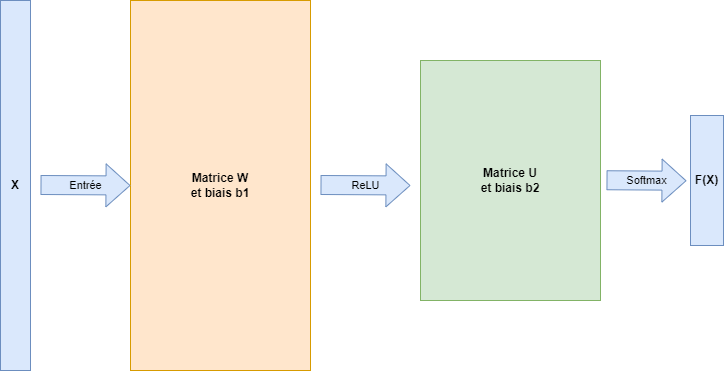
\includegraphics[width=0.60\linewidth]{model1.png}
    \caption{Modèle initiale}
    \label{fig:model1}
\end{figure}

Pour entraîner le modèle, nous avons comparer notre sortie au mot à prédire dans le format One-hot encoding
\footnote{Le format One-hot encoding est un encodage des indices en un vecteur d'une taille du nombre d'indice possible tel que ce vecteur possède des 0 partout sauf à l'indice en question qui possède un 1.}, et nous appliquons le calcule de la fonction de coût: cross-entropy. 
On avons utilisé Adam~\cite{kingma2014adam} pour optimiser les paramètres avec un learning rate de $0.01$ pour les 5 premières époques et $0.001$ pour les suivantes.

\paragraph{Métriques}
Nous avons par ailleurs décidé d'évaluer ce réseau à l'aide de plusieurs métriques comme l'accuracy, la perplexité, le $f_1$-score et la métrique top~$k$\footnote{La métrique "top-$k$" évalue un modèle en comptant combien de prédictions correctes il fait parmi les $k$ premières prédictions les plus probables. Attention ici $k$ n'est pas le nombre de mots dans le contexte!} (avec $k=5$), voir~\cite{DBLP:journals/corr/LiuDLZ15}.

\paragraph{Résultats}

Sur la Figure~\ref{subfig:result model 1}, on voit les courbes d'apprentissage. Les valeurs des métriques sur les données d'entraînement sont en bleue, sur les données de validations sont en orange.
% commenter les courbes

\begin{figure}[ht]
  \centering
  \begin{subfigure}{0.47\textwidth}
    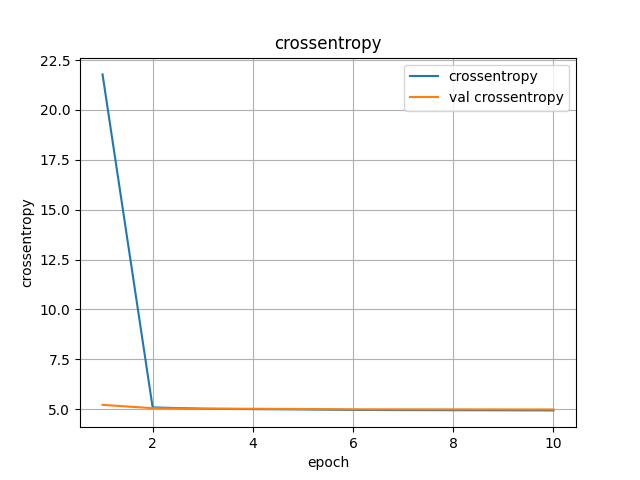
\includegraphics[width=\linewidth]{../logs/word2vect/crossentropy.png}
    \caption{Cross Entropy Loss (Lower is Better)}
  \end{subfigure}
  \hfill
  \begin{subfigure}{0.47\textwidth}
    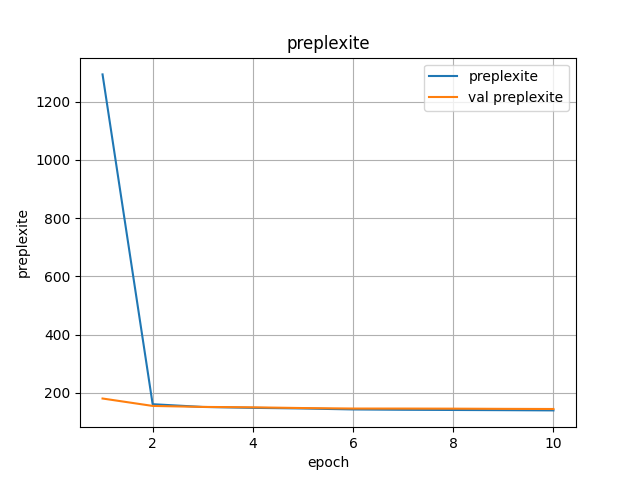
\includegraphics[width=\linewidth]{../logs/word2vect/preplexite.png}
    \caption{perplexité (Lower is Better)}
  \end{subfigure}

  \begin{subfigure}{0.47\textwidth}
    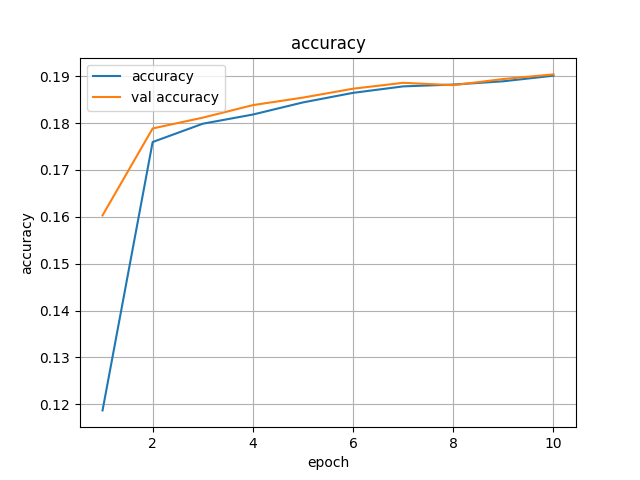
\includegraphics[width=\linewidth]{../logs/word2vect/accuracy.png}
    \caption{Accuracy (Higher is Better)}
  \end{subfigure}
  \hfill
  \begin{subfigure}{0.47\textwidth}
    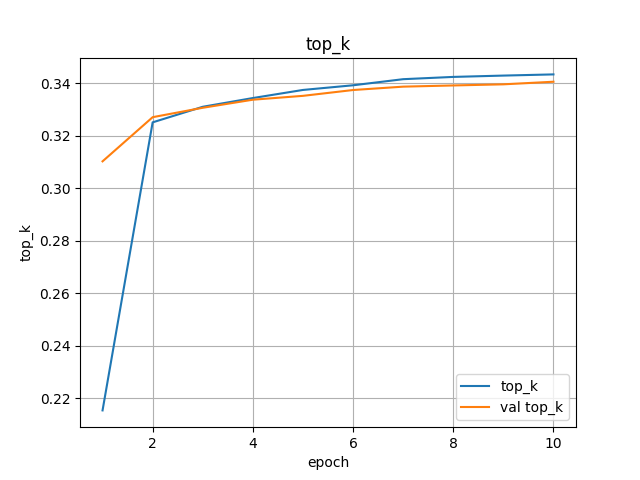
\includegraphics[width=\linewidth]{../logs/word2vect/top_k.png}
    \caption{top k, avec k=5 (Higher is Better)}
  \end{subfigure}
  \caption{Entraînement du modèle initiale}
  \label{subfig:result model 1}
\end{figure}


\subsection{Piste à creuser 1~: Apprentissage automatique des embeddings par le modèle de langage.}

\subsubsection{Description}

%%Décrire ici les idées générales de la piste à creuser. Décrire ensuite les hypothèses que vous cherchez à valier ou invalider.
%%Vous pouvez par exemple dire que vous pensez qu'introduire une modification $X$%% va avoir un effet $E$. Expliquez pourquoi, indépendamment de toute expérience.
%%Il est important que vous soyez le plus explicite possible quant aux hypothèses.

Cette première piste que nous avons exploré consiste à se dire que notre modèle d'embeddings pré-entraîné n'est pas forcément pertinent pour la tâche de prédiction du mot suivant d'une phrase. L'idée est donc de considérer que la matrice d'embeddings peut-être apprise par le modèle de langage et que la matrice apprise sera plus pertinente qu'une matrice apprise séparément pour résoudre la tâche. On va donc considérer que les paramètres de la matrice sont des paramètres apprenables du modèle de langage et donc étendre jusqu'à eux l'algorithme de rétro-propagation du gradient.

\subsubsection{Mise en \oe uvre}

%%Dire ce que vous avez du changer au modèle de base pour prendre en compte vos modifications, les problèmes auxquels vous avez été confrontés et les solutions que vous avez trouvé pour y remédier.

Il a fallut adapter un peu notre code car avant pour avoir l'embedding d'un mot $i$, on utilisé $E[i]$, où $E \in \mathcal{M}_{V, e}(\mathbb{R})$ est la matrice d'embedding. Cependant, cette opération n'est pas dérivable, donc il a fallut transformer le mot $i$ en un vecteur $x \in \mathbb{R}^V$ one-hot, et faire $x \times E$ pour obtenir l'embedding du mots $i$, qui cette fois ci, est une opération dérivable. 
Une fois cette adaptation faite, on a rajouté cette opération dans notre modèle et nous obtenons donc un nouveau modèle illustré par la Figure~\ref{fig:model2}, et donné par l'équation~\eqref{eq:model2}.


\begin{flalign}
    & F(x)=softmax(U(ReLU(W\tilde{X}+b_1))+b_2) \label{eq:model2} & \\
    & \quad \text{où } \tilde{X}=flatten(XE)  \quad \text{et} \quad X \in \mathcal{M}_{k, V}(\mathbb{R}) \notag &
\end{flalign}

\begin{figure}
    \centering
    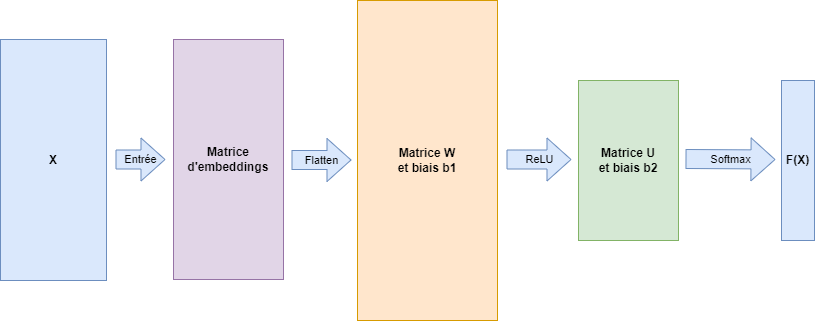
\includegraphics[width=0.60\linewidth]{model2.png}
    \caption{Nouveau modèle avec l'apprentissage des embeddings}
    \label{fig:model2}
\end{figure}


\subsubsection{Résultats}

Décrire les résultats que vous avez obtenu. Dites si vos hypothèses ont été vérifiées. cf subfig:\ref{subfig:result model 2}

Si c'est le cas, donnez des exemples qui le montre.

Si ce n'est pas le cas, faire une analyse des erreurs, proposez des explications et si possible mettez les en \oe uvre dans le cas d'une nouvelle expérience. Souvent, les choses ne marchent pas du premier coup.

\begin{figure}[ht]
  \centering
  \begin{subfigure}{0.47\textwidth}
    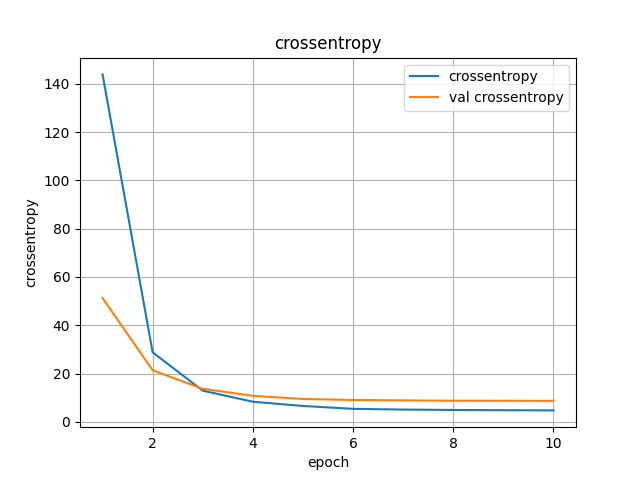
\includegraphics[width=\linewidth]{../logs/learnfromscratch/crossentropy.png}
    \caption{Cross Entropy Loss (Lower is Better)}
  \end{subfigure}
  \hfill
  \begin{subfigure}{0.47\textwidth}
    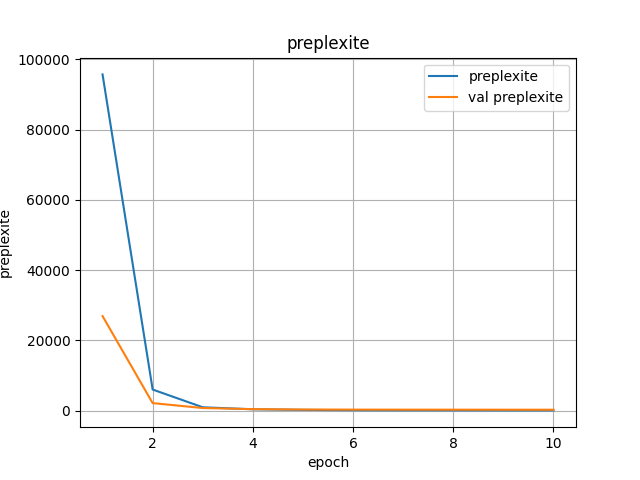
\includegraphics[width=\linewidth]{../logs/learnfromscratch/preplexite.png}
    \caption{perplexité (Lower is Better)}
  \end{subfigure}

  \begin{subfigure}{0.47\textwidth}
    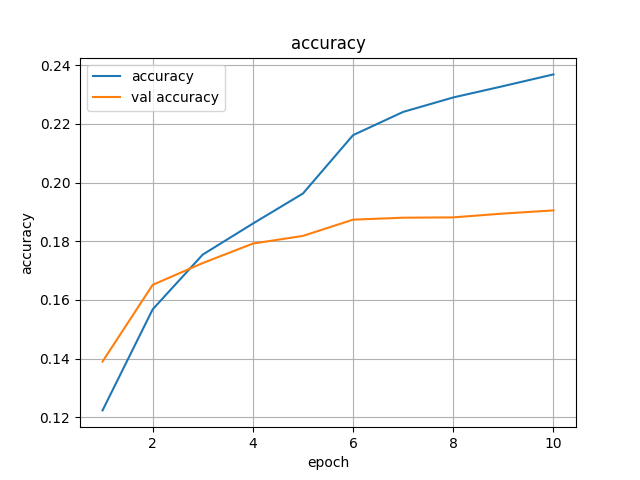
\includegraphics[width=\linewidth]{../logs/learnfromscratch/accuracy.png}
    \caption{Accuracy (Higher is Better)}
  \end{subfigure}
  \hfill
  \begin{subfigure}{0.47\textwidth}
    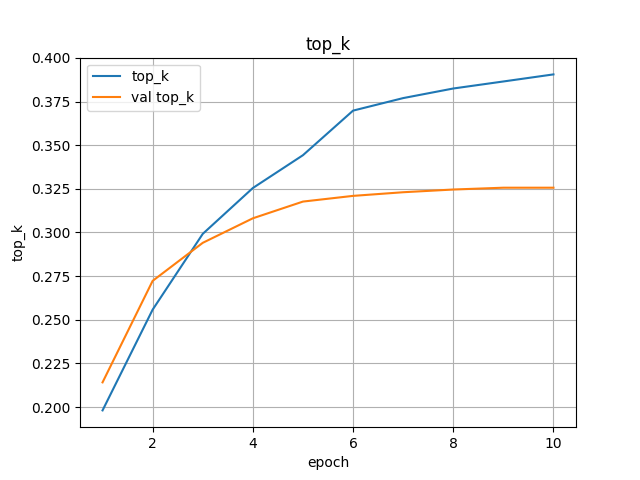
\includegraphics[width=\linewidth]{../logs/learnfromscratch/top_k.png}
    \caption{top k, avec k=5 (Higher is Better)}
  \end{subfigure}
  \caption{Entraînement du modèle avec l'apprentissage des embeddings}
  \label{subfig:result model 2}
\end{figure}


\subsection{Piste à creuser 2~: titre}

même structure

\begin{figure}[ht]
  \centering
  \begin{subfigure}{0.47\textwidth}
    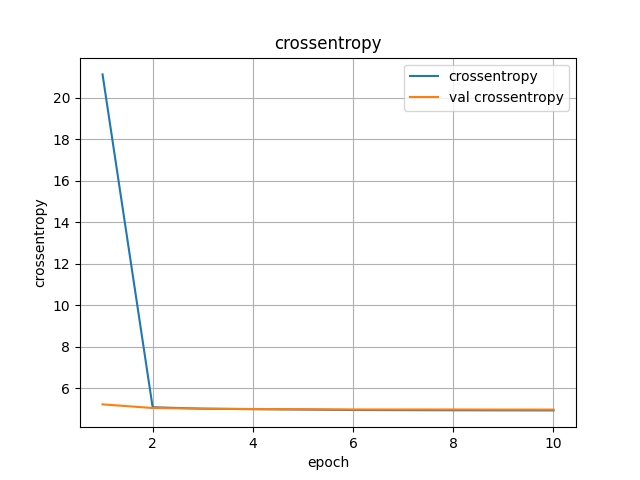
\includegraphics[width=\linewidth]{../logs/learnfromword2vect/crossentropy.png}
    \caption{Cross Entropy Loss (Lower is Better)}
  \end{subfigure}
  \hfill
  \begin{subfigure}{0.47\textwidth}
    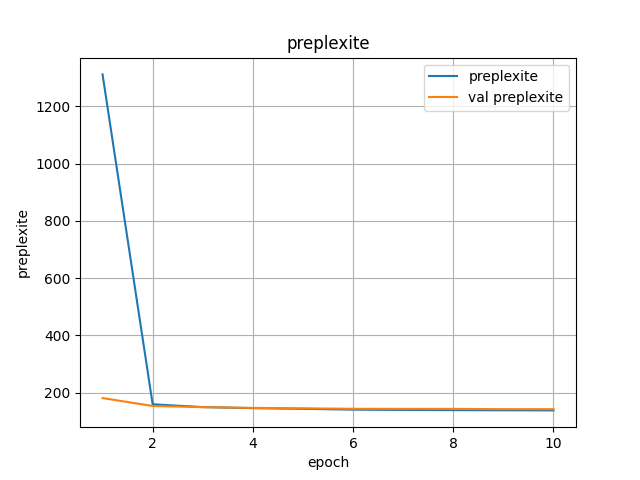
\includegraphics[width=\linewidth]{../logs/learnfromword2vect/preplexite.png}
    \caption{perplexité (Lower is Better)}
  \end{subfigure}

  \begin{subfigure}{0.47\textwidth}
    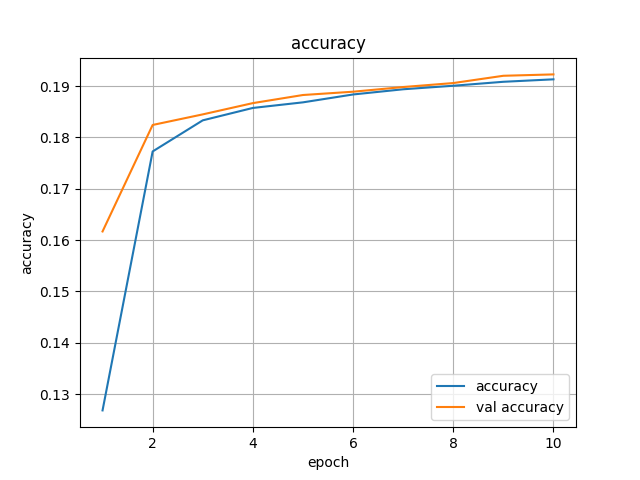
\includegraphics[width=\linewidth]{../logs/learnfromword2vect/accuracy.png}
    \caption{Accuracy (Higher is Better)}
  \end{subfigure}
  \hfill
  \begin{subfigure}{0.47\textwidth}
    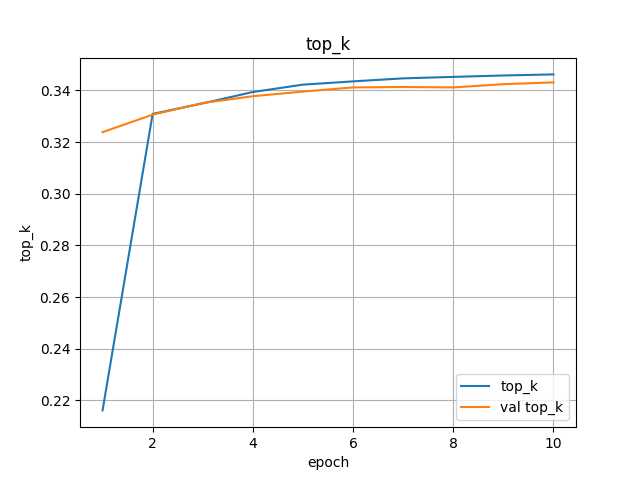
\includegraphics[width=\linewidth]{../logs/learnfromword2vect/top_k.png}
    \caption{top k, avec k=5 (Higher is Better)}
  \end{subfigure}
  \caption{Entraînement du modèle avec l'apprentissage des embeddings à partir des embeddings de Word2Vect}
  \label{subfig:result model 3}
\end{figure}


\section{Conclusions et perspectives}

Reprendre le problème sur lequel vous vous êtes intéressé. Décrire les hypothèses sur lesquelles vous avez travaillé. Revenez sur les résultats que vous avez obtenu et mettant en avant les points qui vous semblent intéressants.

Dites à l'issue de ce travail quelle pistes pourraient être explorées pour aller plus loin.

\begin{table}
    \centering
    \begin{tabular}{|c|c|c|c|c|c|}
        \hline
        métriques & cross entropie & accuracy & top $k$ & $f_1$ score & perplexité \\
        \hline
        modèle initial & $4.89$ &  $0.20$ & $0.35$ & $9.42e-4$ & $131$ \\
        modèle 2 & $8.29$ &  $0.20$ & $0.33$ & $1.10e-3$ & $270$ \\
        modèle 3 & $4.89$ &  $0.20$ & $0.35$ & $8.86e-4$ & $130$ \\
        \hline
    \end{tabular}
    \caption{Résultat des différents modèles sur la base de données de teste}
    \label{tab:allresults}
\end{table}


\begin{table}
    \centering
    \begin{tabular}{|c|c|c|c|}
        \hline
        modèles & 1 & 2 & 3 \\
        \hline
        temps (en s) & 360 & 1001 & 460 \\
         \hline
    \end{tabular}
    \caption{Comparaison du temps d'entraînement des différents modèles sur 10 époques.}
    \label{tab:times}
\end{table}


\newpage

\printbibliography



\end{document}
